\documentclass[11pt]{article}
\usepackage{matt}
\begin{document}

\section*{Update for the Week of \today}

\begin{figure}[h]
  \centering
  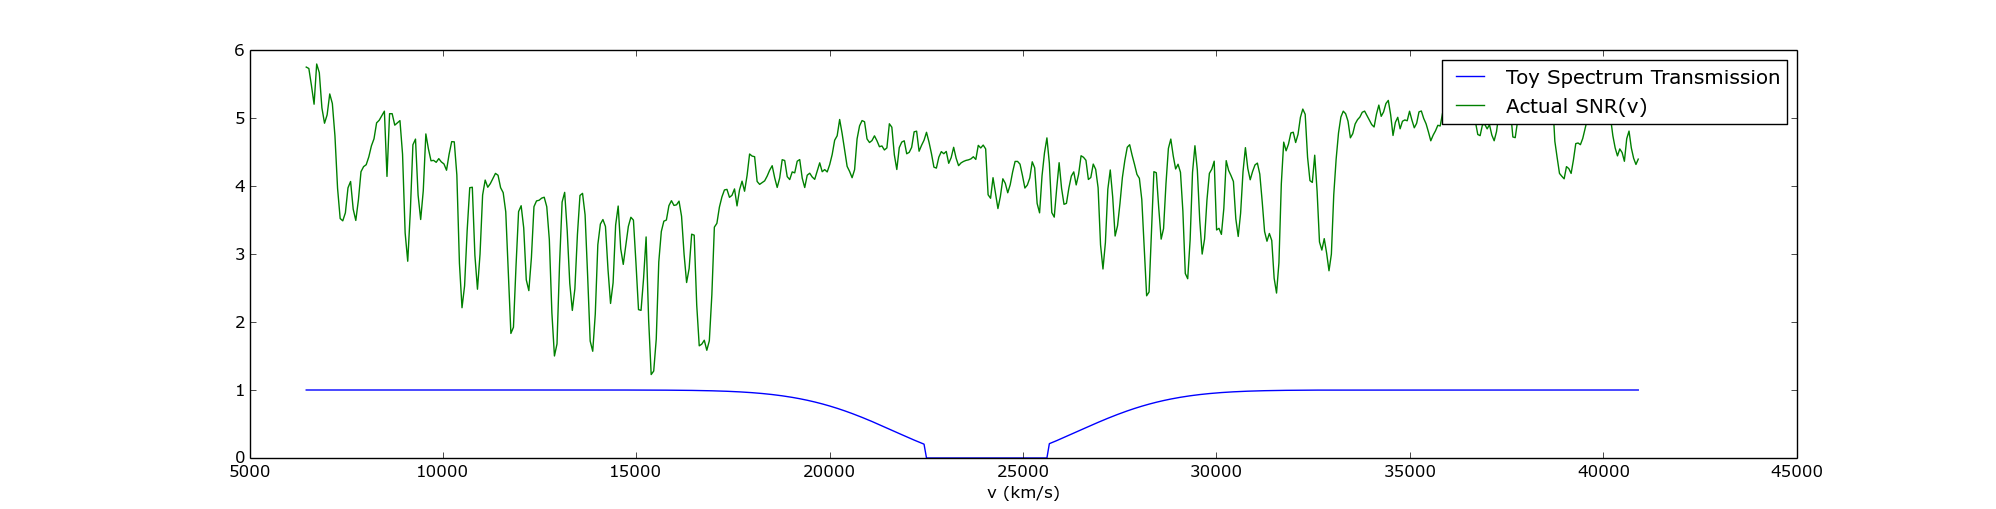
\includegraphics[width=18cm]{ToyFlux_RealNoise.png}
  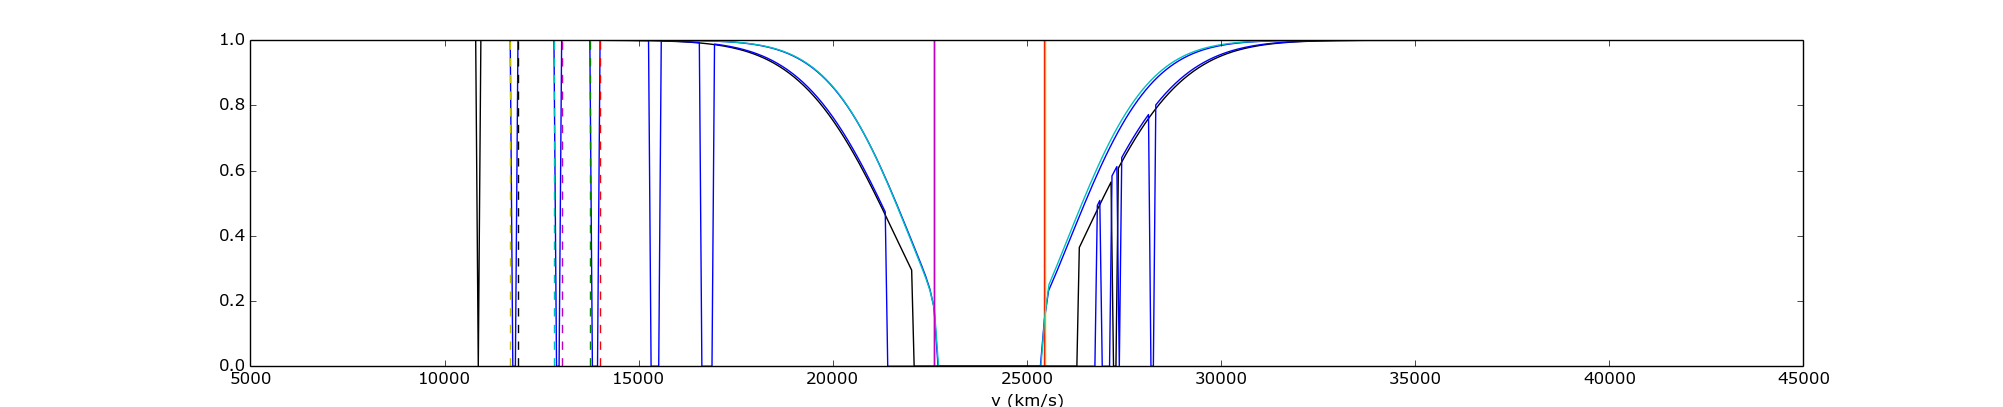
\includegraphics[width=18cm]{ToySpectrum_StackingLocations.png}
  \caption{The top figure shows a toy spectrum (blue) created to test the stacking code, along with a sample $\mathcal{S}(v)$ plot for a spectrum (green). The bottom panel shows the cumulative result of plotting the smoothed spectra along with the identified stacking locations. One feature that we see here is that dips in the signal-to-noise ratio in the above plot correspond to erroneous stacking locations in the bottom plot. In fact, \textit{despite the smoothed transmission being unity}, we are still forced to stack at locations where the signal to noise dips. This is a behavior we should probably find a way to avoid (not difficult to do, probably).}
  \label{fig:todo}
\end{figure}

\begin{figure}[h]
  \centering
  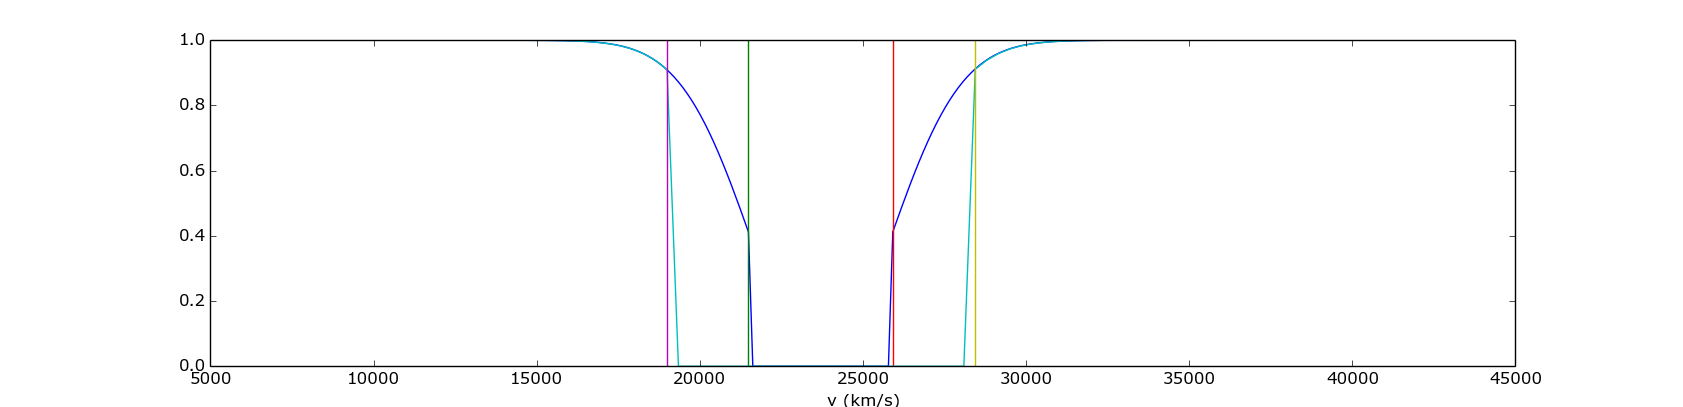
\includegraphics[width=18cm]{ToySpectrum_StackingLocations_HiNoise.png}
  \caption{The above figure (is a mess but) shows two toy spectra with corresponding stacking locations. The cyan smoothed spectrum has $\tilde{F}(v) < 0.9$ consistent with saturated absorption. Maybe we should be disregarding dark gaps coincident with un-usable signal-to-noise values. }
  \label{fig:todo}
\end{figure}

\begin{figure}[h]
  \centering
  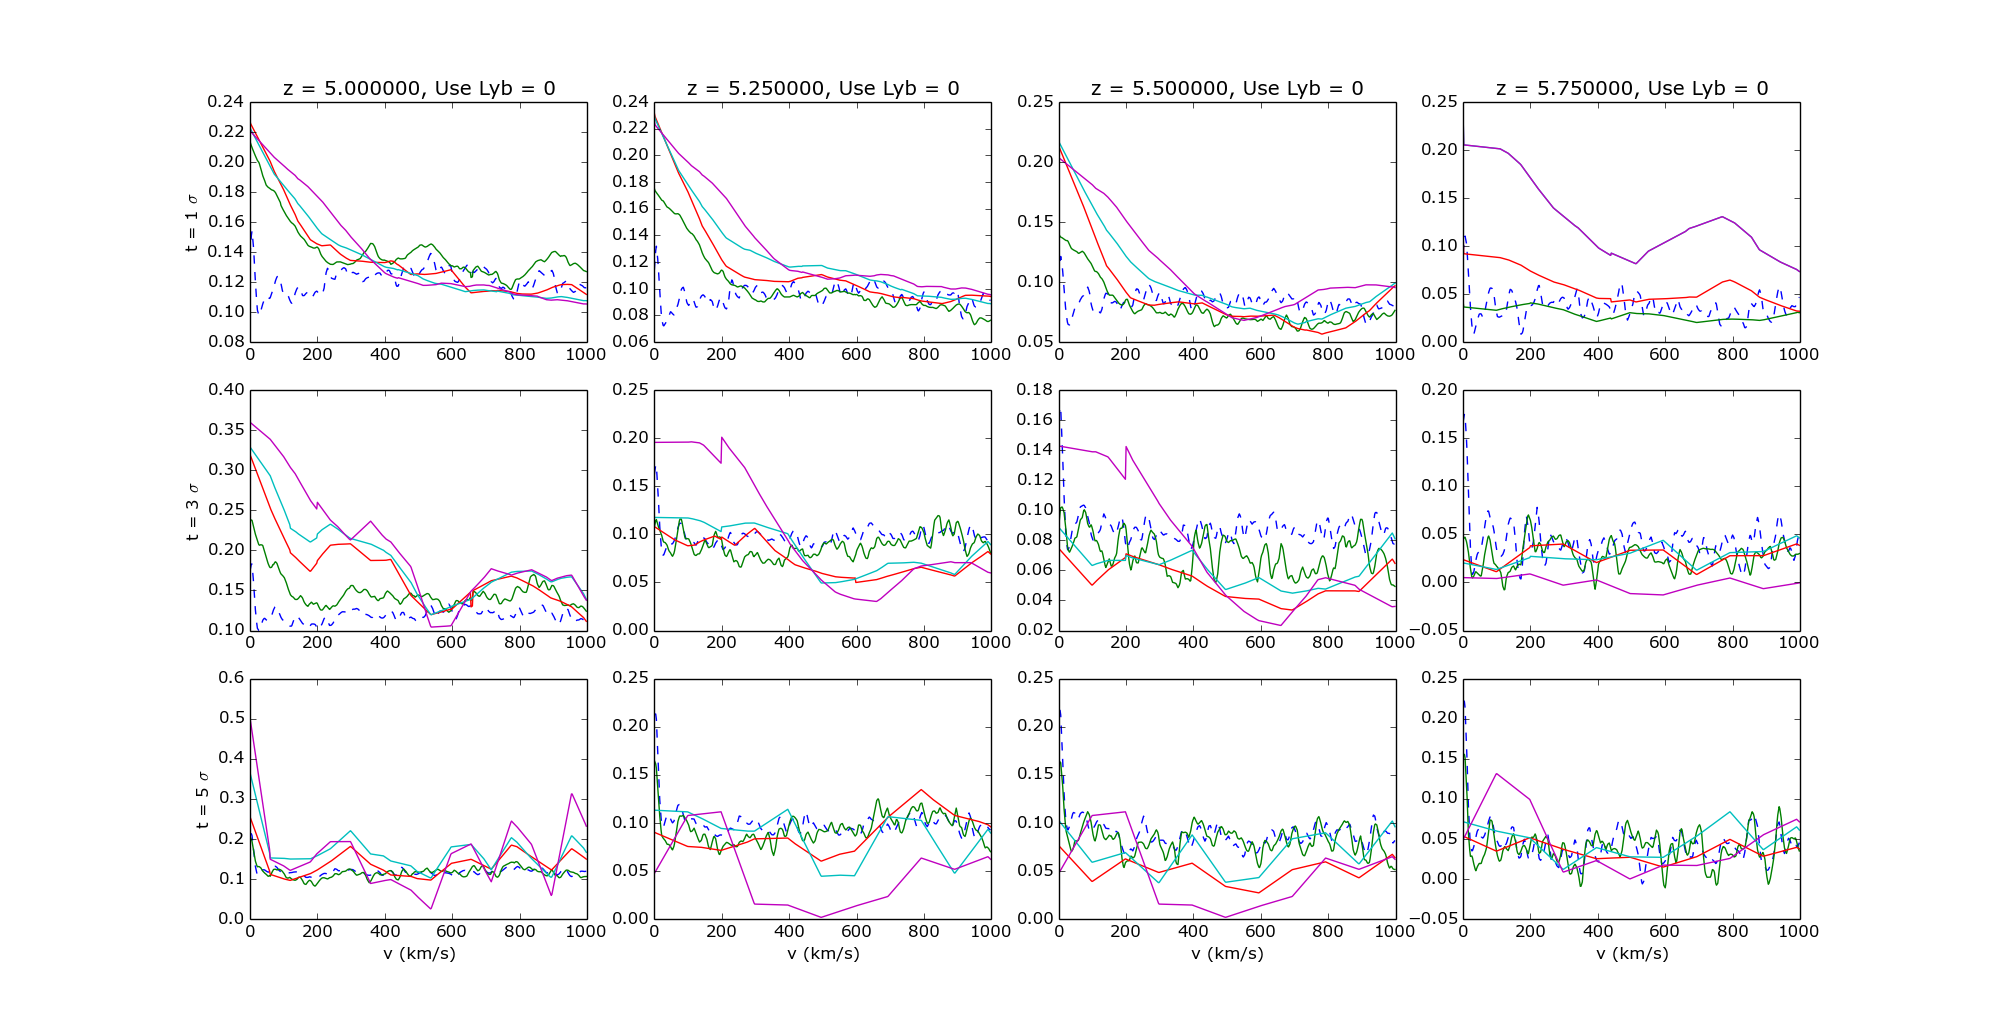
\includegraphics[width=18cm]{GridPlot_Debugged.png}
  \caption{Debugged grid plot.}
  \label{fig:todo}
\end{figure}

\begin{figure}[h]
  \centering
  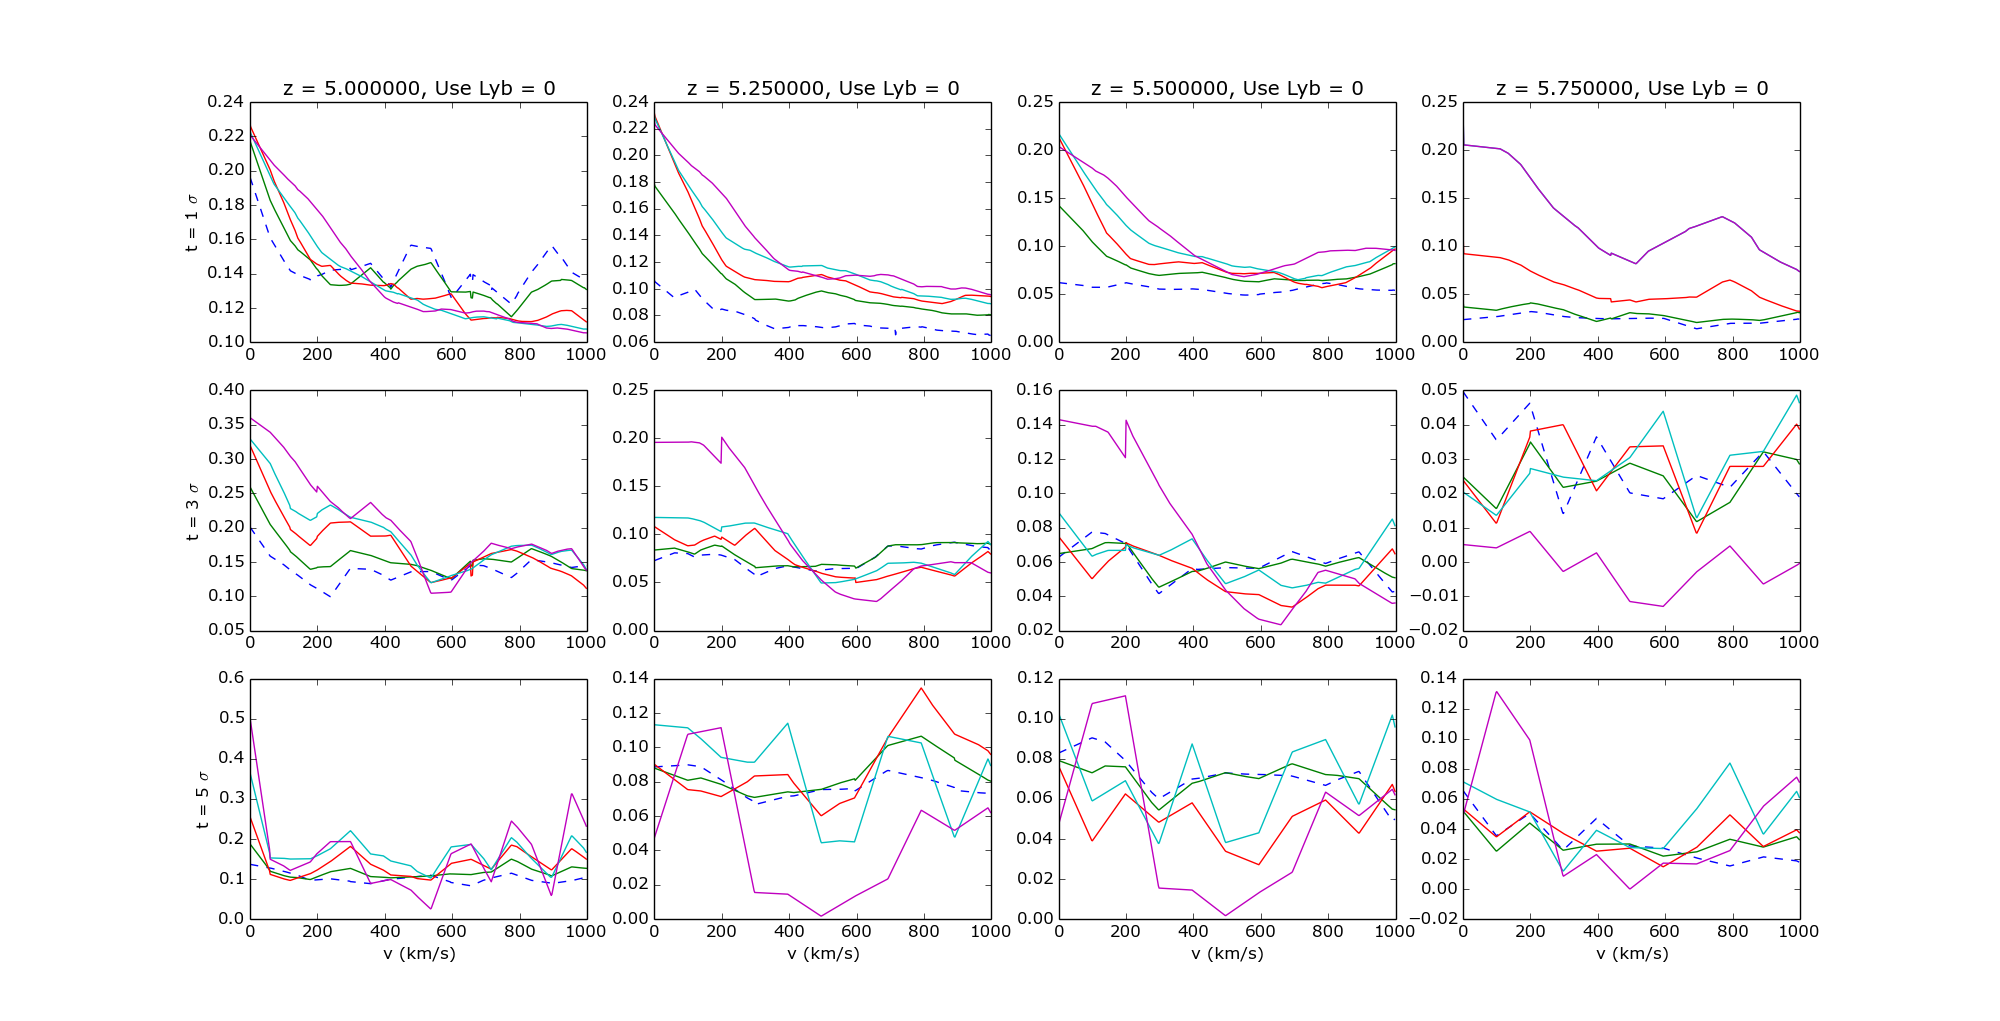
\includegraphics[width=18cm]{GridPlot_Debugged_No10.png}
  \caption{Debugged grid plot, no spectra \# 10}
  \label{fig:todo}
\end{figure}


\begin{figure}[h]
  \centering
  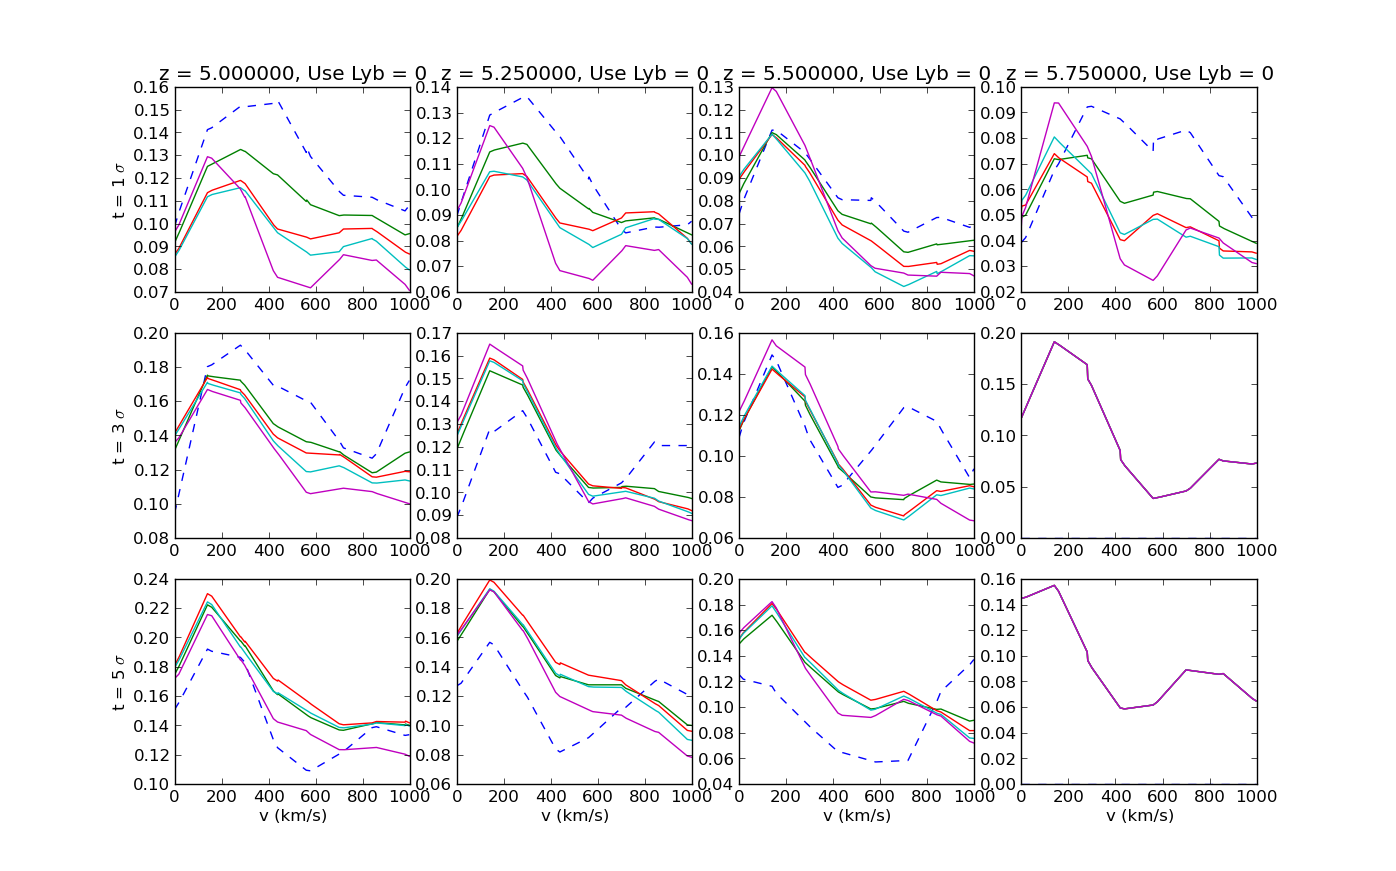
\includegraphics[width=18cm]{gridPlot_CommonRes.png}
  \caption{todo}
  \label{fig:todo}
\end{figure}

\begin{figure}[h]
  \centering
  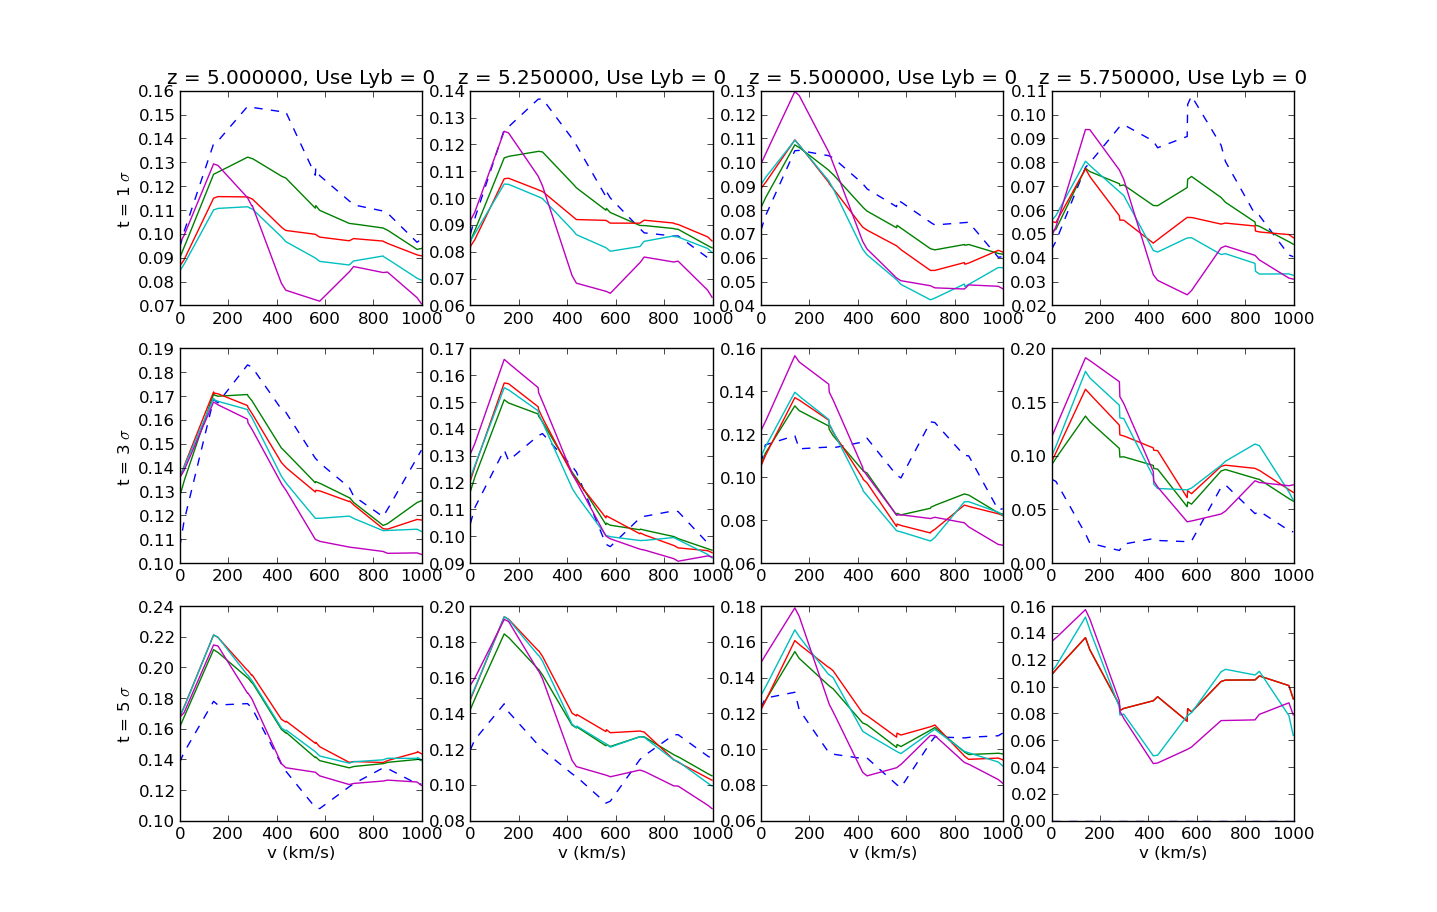
\includegraphics[width=18cm]{gridPlot_CommonRes_AllSpectra.png}
  \caption{todo}
  \label{fig:todo}
\end{figure}

\begin{figure}[h]
\subsubsection*{Suspicious Behavior from $z = 5.99$ Spectrum}
  \centering
  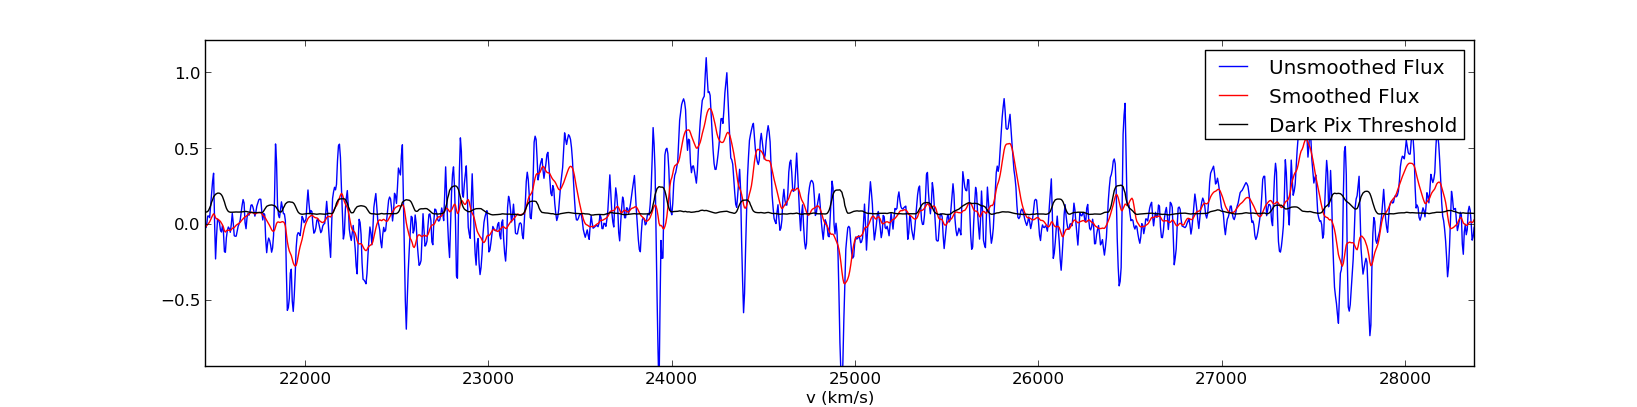
\includegraphics[width=18cm]{z599_Spectra.png}
  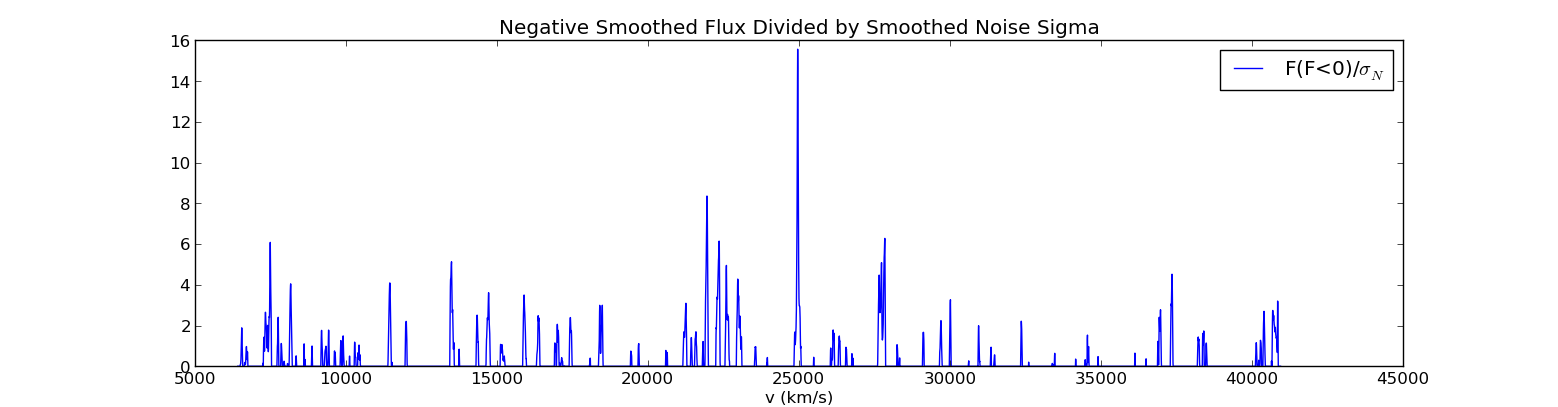
\includegraphics[width=18cm]{z599_NoiseSignificance.png}
  \caption{The top panel shows the unsmoothed spectrum (blue), smoothed spectrum (red) and dark-pixel threshold (black) for the $z = 5.99$ spectrum. The dark-pixel threshold is defined to be $3\tilde{\sigma}_{\text{N}}$. The bottom panel shows negative values in the smoothed spectrum \textit{in units of $\tilde{\sigma}_{\text{N}}$}. From this figure, it seems that negative noise fluctuations in the smoothed spectrum are frequently in excess of $6\tilde{\sigma}_{\text{N}}$.}
  \label{fig:z599}
\end{figure}

\begin{figure}[h]
\subsubsection*{$z = 6.28$ Spectrum}
  \centering
  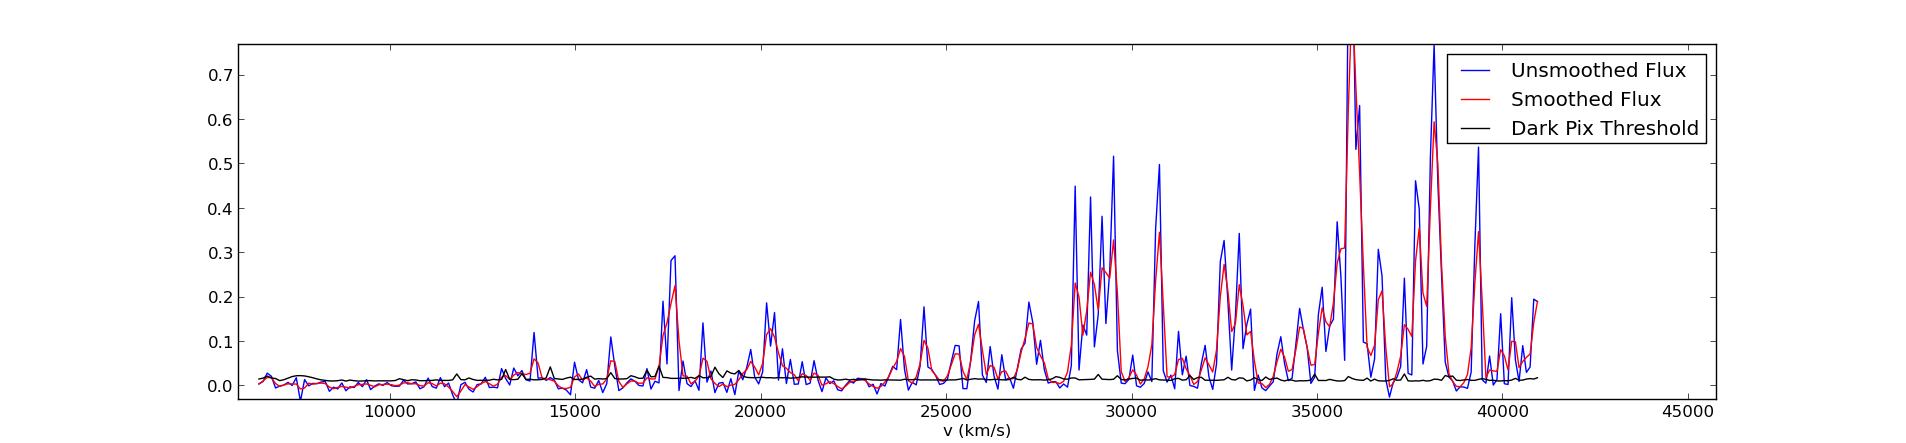
\includegraphics[width=18cm]{z628_Spectra.png}
  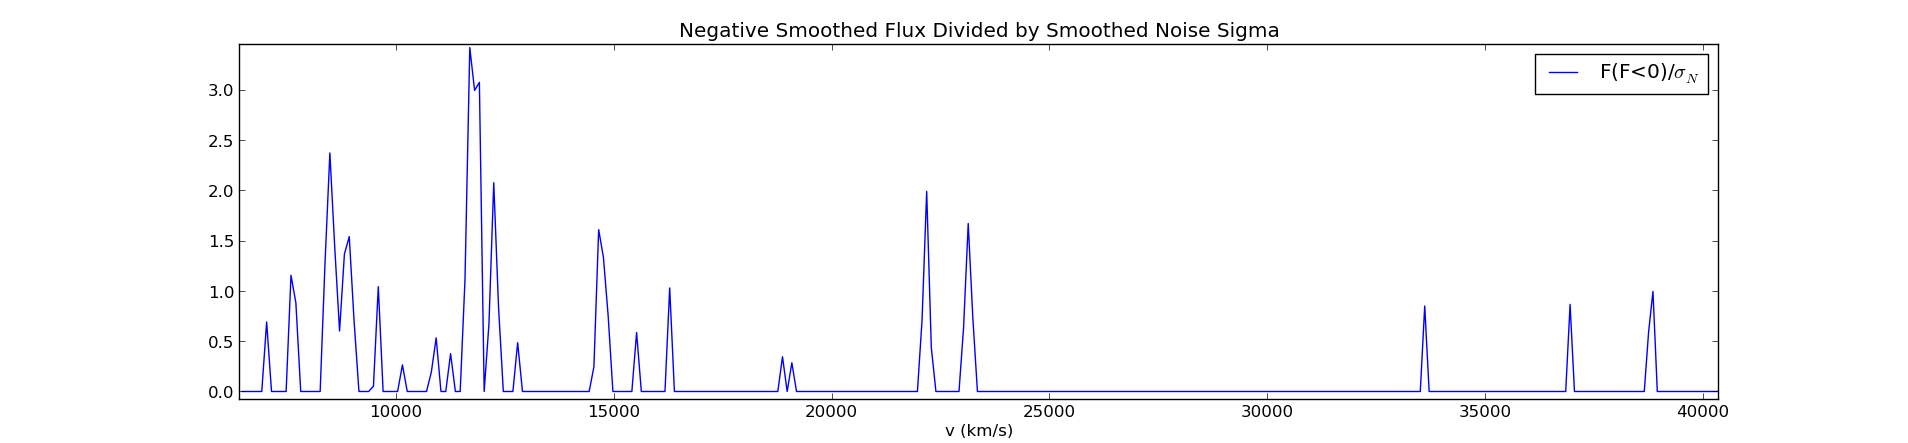
\includegraphics[width=18cm]{z628_NoiseSignificance.png}
  \caption{This figure is the same as Figure \ref{fig:z599}, except for a spectrum with $z_{\text{QSO}} = 6.28$. This spectrum doesn't display suspicious behavior during stacking. It also does not display curiously large downward fluctuations in the noise.}
  \label{fig:todo}
\end{figure}



\end{document}